The main results of the thesis are differential cross-section measurements at the particle level. The inclusive detector level cross-section for a given physics process $p_{1}p_{2}\rightarrow X$ is, 

\begin{equation}
    \sigma ^{detector~level}_{p_{1}p_{2}\rightarrow X} = A \times \epsilon \times \sigma ^{particle-level}_{p_{1}p_{2}\rightarrow X}
    \label{eqn:InclusiveXS}
\end{equation}
where $\sigma ^{particle-level}_{p_{1}p_{2}\rightarrow X}$ is the \textit{true} cross-section of the physics process predicted by the theory. The physical layout of the ATLAS detector does not cover all areas of the phase space. $A$ accounts for the limited acceptance of the ATLAS detector. Several parts of the detector have several reconstruction efficiencies, which are accounted for by the factor $\epsilon$. The detector level cross-section is measured experimentally in terms of the number of particles in a given final state (N) and integrated Luminosity $L$ as $\sigma ^{detector~level}_{p_{1}p_{2}\rightarrow X} = \frac{N}{L}$. The \textit{true} particle level inclusive cross-section can be estimated by correcting for detector acceptance and detector efficiency for the measured cross-section $\sigma ^{detector~level}_{p_{1}p_{2}\rightarrow X}$.

For differential cross-sections where the cross-section is measured in different bins of the kinematic observables, additional correction is needed to correct the resolution-induced migration between nearby bins. 

This Chapter discusses the unfolding technique in detail. Section \ref{subsec:UnfoldingOverview} gives an Overview on the unfolding algorithm, whereas Section \ref{subsec:UnfoldingValidation} validates the unfolding method. Section \ref{subsec:Bias} discusses the bias from unfolding and the attempts to optimize the bias.  

\subsection{Method Overview}
\label{subsec:UnfoldingOverview}
The analysis uses an \textit{iterative Bayesian unfolding} algorithm based on Baye's theorem \cite{BayesianUnfolding} \cite{Improved_BayesianUnfolding} using ATLAS-supported \textit{RooUnfold} package \cite{RooUnfold}. Bayes' theorem formulates a mathematical relation to obtain a probability of an effect $E$ caused by several independent causes $C_{i}$, given the initial probability of the causes $P(C_{i})$ and the conditional probability of the $i-th$ cause to produce the effect $P(E|C_{i})$ as, 

\begin{equation}
P(C_{i}|E) = \frac{ P(E|C_{i}) . P(C_{i}) } { \sum_{j}{ P(E|C_{j}).P(C_{j}) } }
\label{eqn:BayesTheorem}
\end{equation}

The obtained probability depends on the prior probability of the cause and the conditional probability of cause and effect. The prior dependency is reduced by using an iterative technique, where the outcome of the previous iteration is used as a prior for the subsequent iteration.

For a single iteration, the algorithm can be summarized as, 

\begin{equation}
    U_{i} = \frac{1}{ \epsilon_{i} } \times \sum^{reco~bins}_{j}{ (R_j -F_j ) . f_{i} . \frac{M_{ji} T_{i}}{ \sum_{k}^{truth~bins}{M_{jk} T_{k}}} } 
    \label{eqn:BayesianUnfolding}
\end{equation}
where $U_{i}$ is the unfolded yield in the target bin $i$, $T_{i}$ is the predicted truth level yield in particle bin $i$, $R_{j}$ is the observed detector level yield in reco bin $j$ and $F_{j}$ is the subtracted detector level reducible background yield. $M_{ij}$ is the migration matrix element from particle level bin $j$ to detector level bin $i$. 

Based on the discussion, conceptually, three corrections from the SM MC prediction need to be applied to estimate the unfolded yield. The three unfolding inputs are 

\begin{itemize}
    \item{\textit{\textbf{Reconstruction efficiency ($\epsilon$):}} The reconstruction efficiency accounts for the limited acceptance and efficiency of the detector. Technically, it is defined as a fraction of events that pass both detector and fiducial level selection to the events passing only the fiducial level selection. }
    
    \item{\textit{\textbf{Fiducial fraction ($f$):}} The fiducial fraction accounts for events that are outside the fiducial region at the particle level, which due to limited detector resolution entered in the measured distribution. An example of such an event would be a signal $4\ell+jj$ event where one of the jets originates from pile-up instead of hard-scatter. Technically, it is defined as a fraction of events that pass both detector and fiducial level selection to the events passing only the detector level selection. }
    
    \item{\textit{\textbf{Migration matrix ($M_{ij}$):}} The migration matrix is a two-dimensional matrix that accounts for events migrated from particle level bin $j$ to detector level bin $i$. The migration matrix corrects the probability of bin migration. It is measured in MC by comparing particle and detector levels distributions for events that pass both fiducial and detector-level selections. Bin migrations result from resolution effects and smearing of the reconstructed distributions. The diagonal component of the migration matrix is related to the \textit{fiducial purity}, which corresponds to the fraction of detector-level events that originate from the same bin at the particle level.}
\end{itemize}

Figure \ref{fig:UnfoldingInputs} show all three unfolding inputs along with the purity as a function of $m_{jj}$. The reconstruction efficiency is less than $50\%$ caused by the poor jet reconstruction efficiency. The fiducial fraction and purity is smaller in lower bins of $m_{jj}$, which mainly corresponds to contribution from pileup jets faking the event selection. The normalized migration matrix shown in the second plot with the particle level prediction in $y-axis$ and the detector level prediction in $x-axis$ is diagonal.

\begin{figure}[htb]
    \centering
    \begin{subfigure}{.48\textwidth}
        \centering
        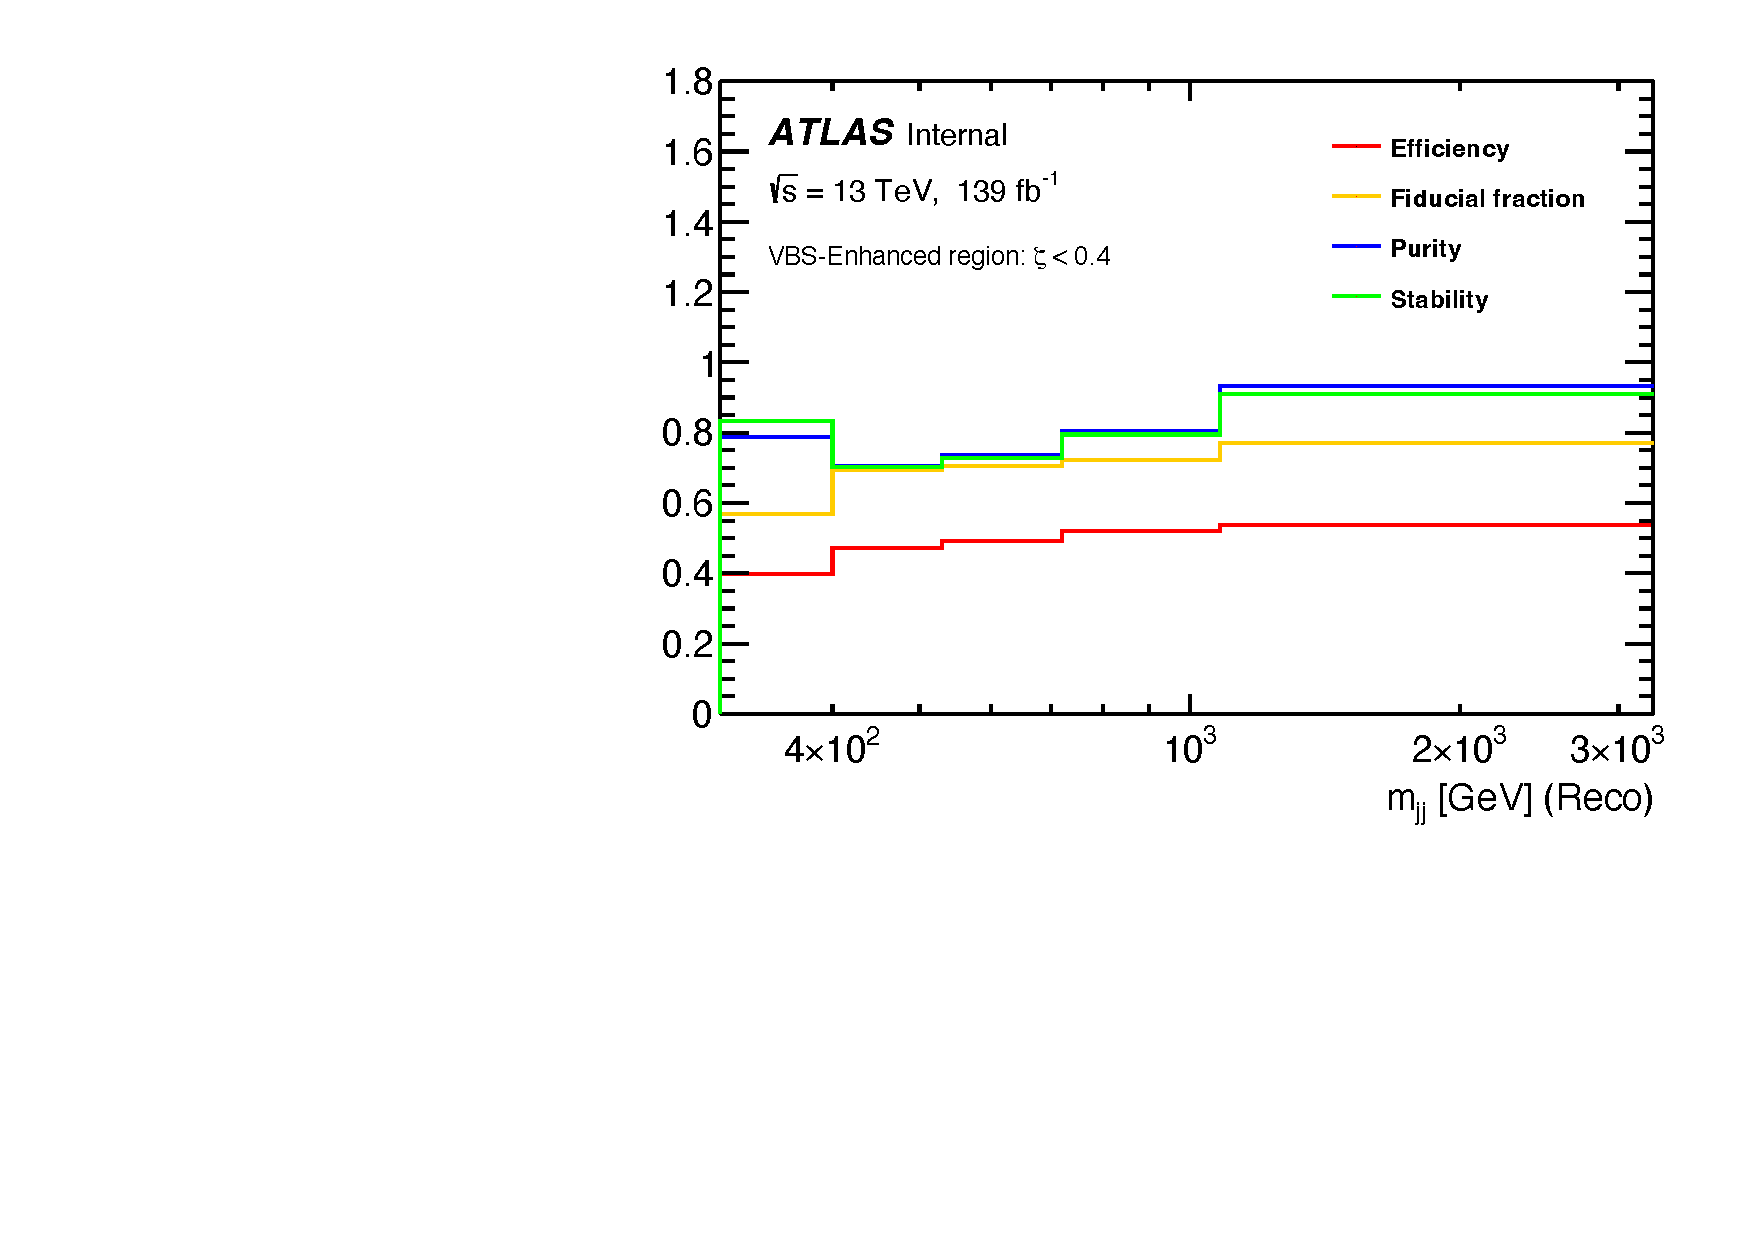
\includegraphics[width=.9\linewidth]{figures/Analysis/Unfolding/efficiencies_VBS_Enhanced.pdf}
        \caption{ reconstruction efficiency (red), fiducial fraction (yellow) and purity (blue). }
    \end{subfigure}
    \begin{subfigure}{.48\textwidth}
        \centering
        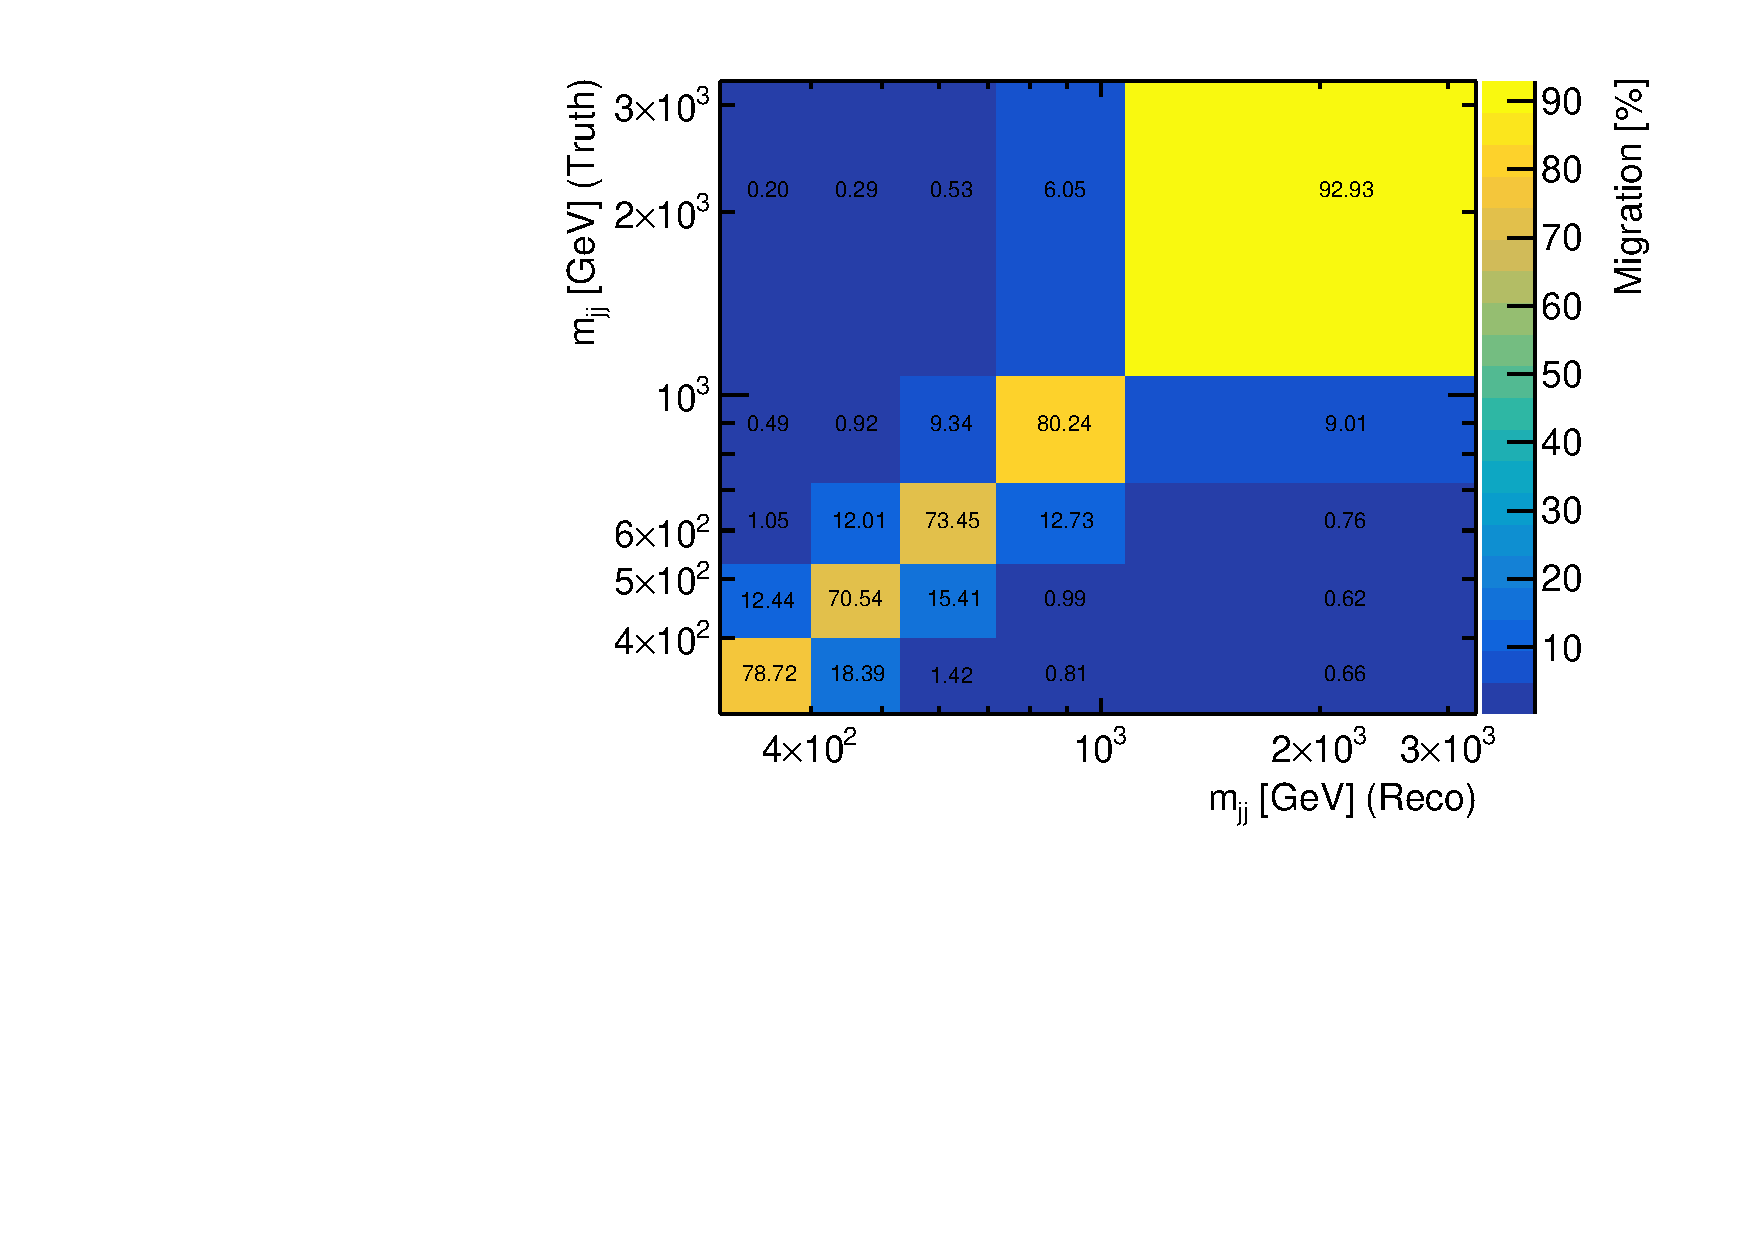
\includegraphics[width=.9\linewidth]{figures/Analysis/Unfolding/migration_matrix_VBS_Enhanced.pdf}
        \caption{migration matrix}
    \end{subfigure}
    \caption{ Unfolding inputs from SM MC as a function of $m_{jj}$.\textcolor{red}{remake first plot with ATLAS Label and stability} \label{fig:UnfoldingInputs}}
\end{figure}

\subsection{Binning for Unfolding}
\label{subsec:Binning}
Choosing optimal binning to perform the unfolding procedure for all kinematic observables effectively is imperative. Two factors drive the choice of binning; first, the necessity to have large enough bin statistics to maintain the Gaussian approximation while preserving the shape of the differential distributions, and second, the necessity to minimize large bin migrations and statistical uncertainties from unfolding. Therefore, each bin must have at least $15$ events in the VBS-Suppressed region and at least $20$ events in the VBS-Enhanced signal region. 

To maintain a good performance of the unfolding, each bin for the kinematic observable has at least $70\%$ purity except for $p_{T,4\ell jj}$ where at least $50\%$ purity is required. Moreover, for each observable, every bin width must be equal to or greater than the resolution of the same bin. The resolution in each particle-level bin is evaluated from MC by comparing the difference of particle and detector level yield for events that pass both fiducial- and detector-level event selection. The difference is fitted using Gaussian approximation, and twice the resulting standard deviation is taken as the resolution. Table \ref{tab:binning} shows the final bin choices for all the kinematic observables used in differential cross-section measurement.
.

\begin{table}
    \caption{Binning for all unfolded observables in VBS-Enhanced and suppressed regions. \label{tab:binning}}
    \begin{center}
    \begin{tabular}{ | c | c | c | }
    \hline
    Observable & Region & Binning \\
    \hline \hline
    \multirow{4}{*}{ $m_{jj}$ [GeV] } &  &  \\
        & VBS-Enhanced & [300, 400, 530, 720, 1080, 3280] \\
    & VBS-Suppressed & [300, 410, 600, 178] \\
    & &\\
    \hline
    \multirow{4}{*}{ $m_{4\ell}$ [GeV] } &  &  \\
        & VBS-Enhanced & [130, 210, 250, 304, 400, 1130] \\
    & VBS-Suppressed & [130, 226, 304, 752] \\
    & &\\
    \hline
    \multirow{4}{*}{ $p_{T,4\ell}$ [GeV] } &  &  \\
    & VBS-Enhanced & [0, 50, 80, 116, 174, 512] \\
    & VBS-Suppressed & [0, 76, 140, 424]\\
    & &\\
    \hline
    \multirow{4}{*}{ $p_{T,jj}$ [GeV] } &  &  \\
    & VBS-Enhanced & [0, 52, 82, 116, 172, 524] \\
    & VBS-Suppressed & [0, 80, 146, 448]\\
    & &\\
    \hline
    \multirow{4}{*}{ $p_{T,4\ell jj}$ [GeV] } &  &  \\
    & VBS-Enhanced & [0, 20, 42, 64, 298] \\
    & VBS-Suppressed & [0, 36, 70, 254]\\
    & &\\
    \hline
    \multirow{4}{*}{ $s_{T,4\ell jj}$ [GeV] } &  &  \\
    & VBS-Enhanced & [70, 240, 320, 420, 580, 1410] \\
    & VBS-Suppressed & [70, 330, 500, 1210]\\
    & &\\
    \hline
    \multirow{4}{*}{ $|\Delta y_{jj}|$ } &  &  \\
    & VBS-Enhanced & [2, 3.08, 3.74, 4.32, 5.06, 7.4] \\
    & VBS-Suppressed & [2, 2.94, 3.78, 5.4]\\
    & &\\
    \hline
    \multirow{4}{*}{ $\Delta \phi_{jj}^{signed}$ } &  &  \\
    & VBS-Enhanced & [$-\pi$, -2.1, 0, 2.1, $\pi$] \\
    & VBS-Suppressed & [$-\pi$,0,$\pi$] \\
    & & \\
    \hline
    \multirow{4}{*}{ $cos \theta_{\ell i\ell j}^{\ast}$ } &  &  \\
    & VBS-Enhanced & [-1, -0.5, 0, 0.5, 1] \\
    & VBS-Suppressed & [-1, 0, 1]\\
    & & \\
    \hline
    \multirow{4}{*}{ $\zeta$ } &  &  \\
    & VBS-Enhanced &[0, 0.06, 0.12, 0.18, 0.26, 0.4] \\
    & VBS-Suppressed & [0.4, 0.5, 0.64, 1.02]\\
    & &\\
    \hline
    \end{tabular}
    \end{center}
\end{table}

\subsection{Method Validation}
\label{subsec:UnfoldingValidation}
The unfolding method is validated using three different tests.

\subsubsection{MC Closure Test}
\label{subsubsec:MCClosure}

The first validation of the unfolding technique is with the SM MC. An SM-predicted detector level distribution for a kinematic observable is unfolded using the unfolding inputs from the same MC. Figure \ref{fig:unfolding_technical_closure} shows an example of the MC-based closure test for $m_{jj}$ in the VBS-Enhanced region. The blue detector-level MC prediction is unfolded using the inputs from the same MC, and the resulting black unfolded distribution is compared with the red particle-level prediction. Since both detector-level prediction and unfolding inputs are from the same MC, a perfect closure between the unfolded and particle-level distribution is observed.

\begin{figure}[!htb]
\centering
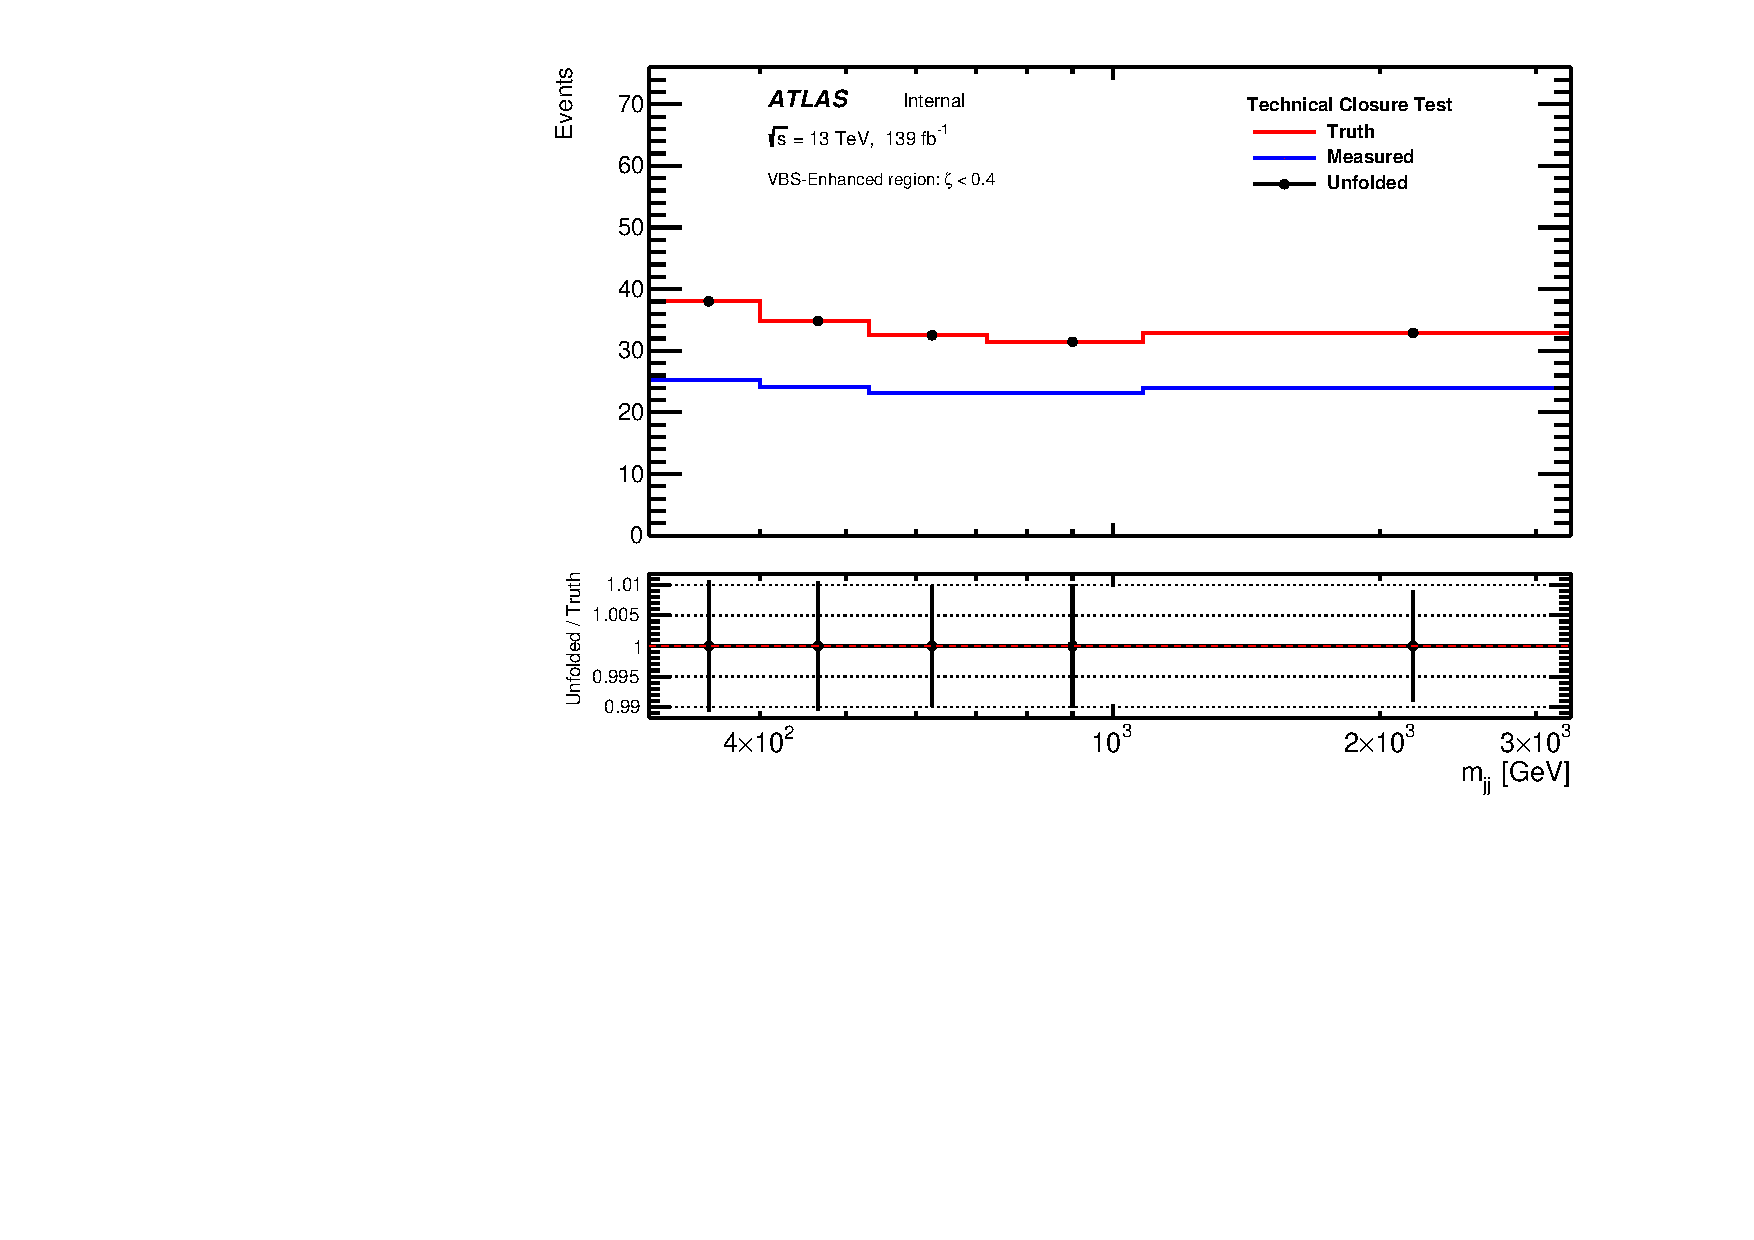
\includegraphics[width=.6\textwidth]{figures/Analysis/Unfolding/technical_closure_VBS_Enhanced.pdf}
\caption{MC technical closure test of the unfolding procedure for $m_{jj}$. The detector-level MC distribution (in blue) is unfolded with the nominal SM unfolding inputs and compared to the particle-level distribution (in red) from the same MC. A perfect closure between unfolded and particle level distribution is observed\label{fig:unfolding_technical_closure}}
\end{figure}

\subsubsection{Injection Test}
\label{subsubsec:InjectionTest}
The analysis uses a model-independent EFT approach discussed in Section \ref{sec:EFT} to constrain the effect of BSM physics. Therefore, it is essential to test the ability of the unfolding algorithm to uncover the accurate particle-level prediction from data containing BSM physics via injection test. In an injection test, a BSM physics contribution is added to the SM detector-level prediction, unfolded with the nominal SM unfolding inputs, and compared with the BSM-added particle-level distribution. Figure \ref{fig:Dim8cont} shows an injection test for $m_{jj}$ in the VBS-Enhanced region where a BSM contribution (green distribution) is added to the SM MC. The BSM contribution is from linear and quadratic contributions of an $FT0$ EFT operator. Figure \ref{fig:InjectTestResult} shows the result of the injection test. The BSM-added detector-level MC prediction (blue) is unfolded (black) using nominal SM MC unfolding inputs and compared against the BSM-added particle-level distribution (red). A small non-closure of about $5\%$ in the last bin of $m_{jj}$ is observed, which is well within the uncertainties of the unfolded distribution.

\textcolor{red}{Note to self: perhaps it makes sense to discuss EFT theory motivation in theory section?}

\begin{figure}[htb]
    \centering
    \begin{subfigure}{.48\textwidth}
        \centering
        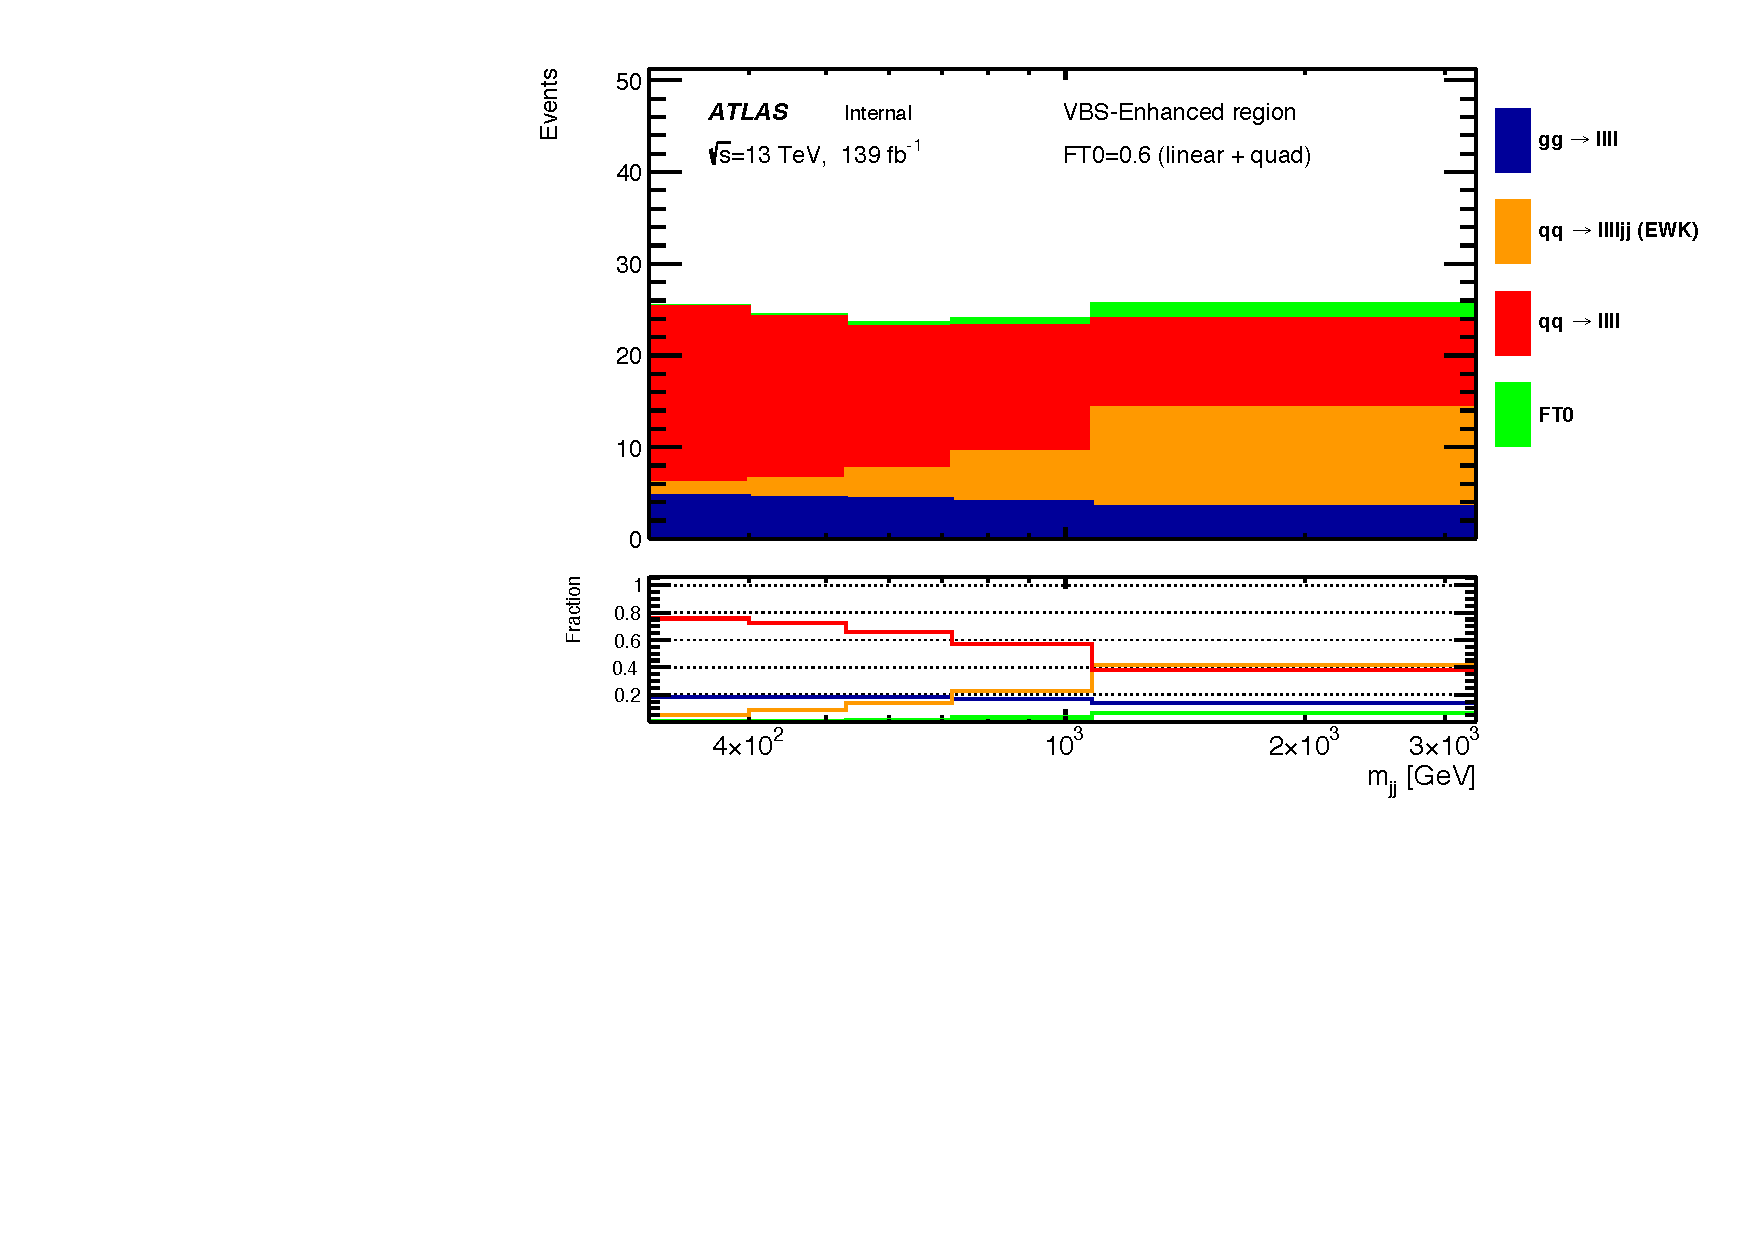
\includegraphics[width=.9\linewidth]{figures/Analysis/Unfolding/injection_test_FT0_quad_mjj_detectorPred.pdf}
        \caption{ Detector level MC prediction with contribution from dimension$-8$ $FT0$ EFT operator. \label{fig:Dim8cont} }
    \end{subfigure}
    \begin{subfigure}{.48\textwidth}
        \centering
        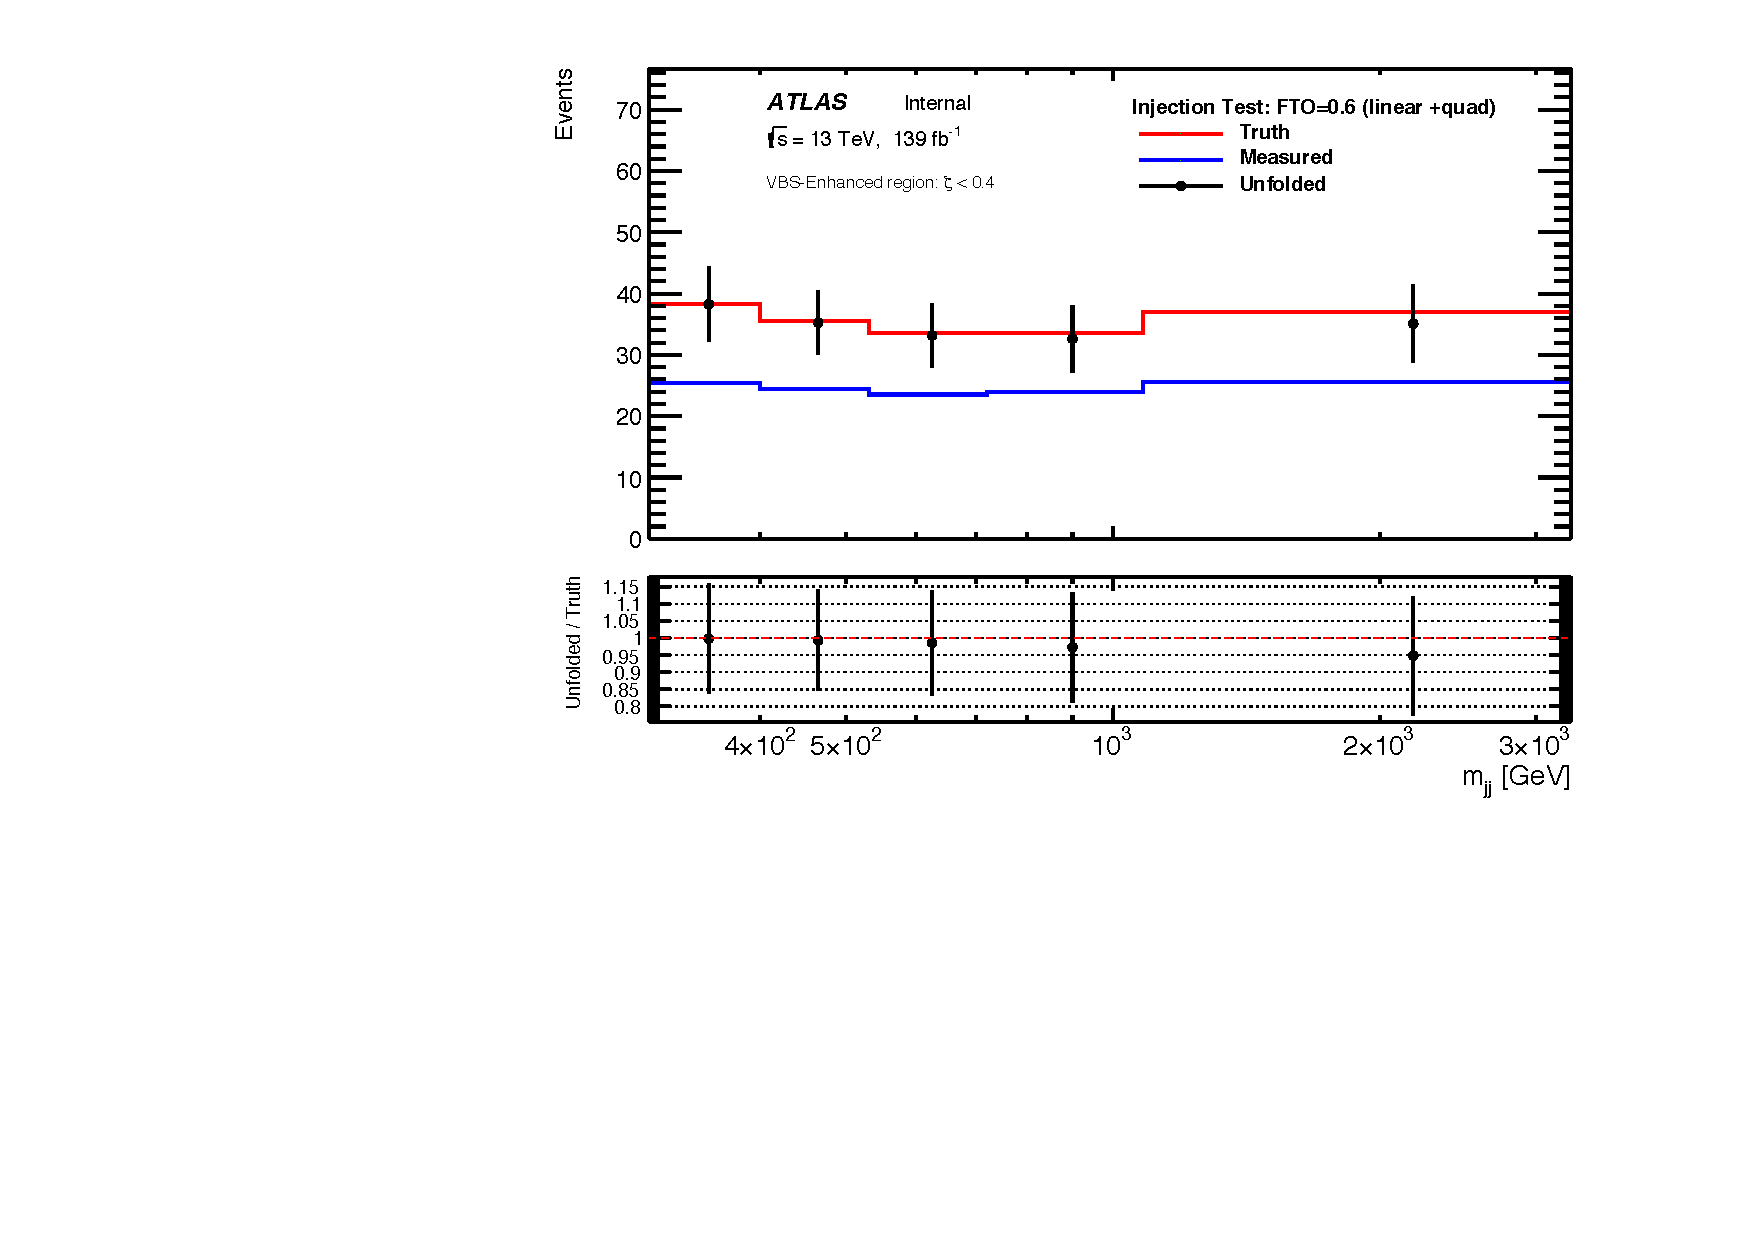
\includegraphics[width=.9\linewidth]{figures/Analysis/Unfolding/injection_test_FT0_quad_mjj.pdf}
        \caption{Unfolded SM+EFT MC detector-level distribution with response matrix from SM MC. \label{fig:InjectTestResult}}
    \end{subfigure}
    \caption{ Injection test with  dimension$-8$ $FT0$ EFT operator. \textcolor{red}{remake plots with ATLAS Label} \label{fig:injection_test_FT0_quad}}
\end{figure}

\subsubsection{Physics Variation}
FFrom the previous ATLAS electroweak $ZZjj$ analysis, a slight enhancement on the central value of the EWk $ZZjj$ cross-section was measured \cite{ATLASZZjj}. The final unfolding validation tested the ability of the algorithm to recover the actual shape of particle-level distribution if a physics process cross-section was different from the SM prediction. First, as shown by figure \ref{fig:unfolding_xsec_var_QCD}, the cross-section for parton-initiated QCD $qqZZjj$ is varied by a factor equal to the total statistical uncertainty on data in the VBS-Suppressed region $\pm  15\%$. The varied detector-level distribution is then unfolded using the nominal SM MC unfolding inputs and compared with the varied fiducial level prediction. Figure \ref{fig:unfolding_xsec_var_EWK} shows the same test where the $EWK qqZZjj$ cross-section is varied by $\pm 11\%$ based on the enhanced cross-section observed in the previous measurement. In both cases, a non-closure of about $1\%$ is observed, well below the uncertainties from unfolding.

\begin{figure}[htb]
    \centering
    \begin{subfigure}{.48\textwidth}
        \centering
        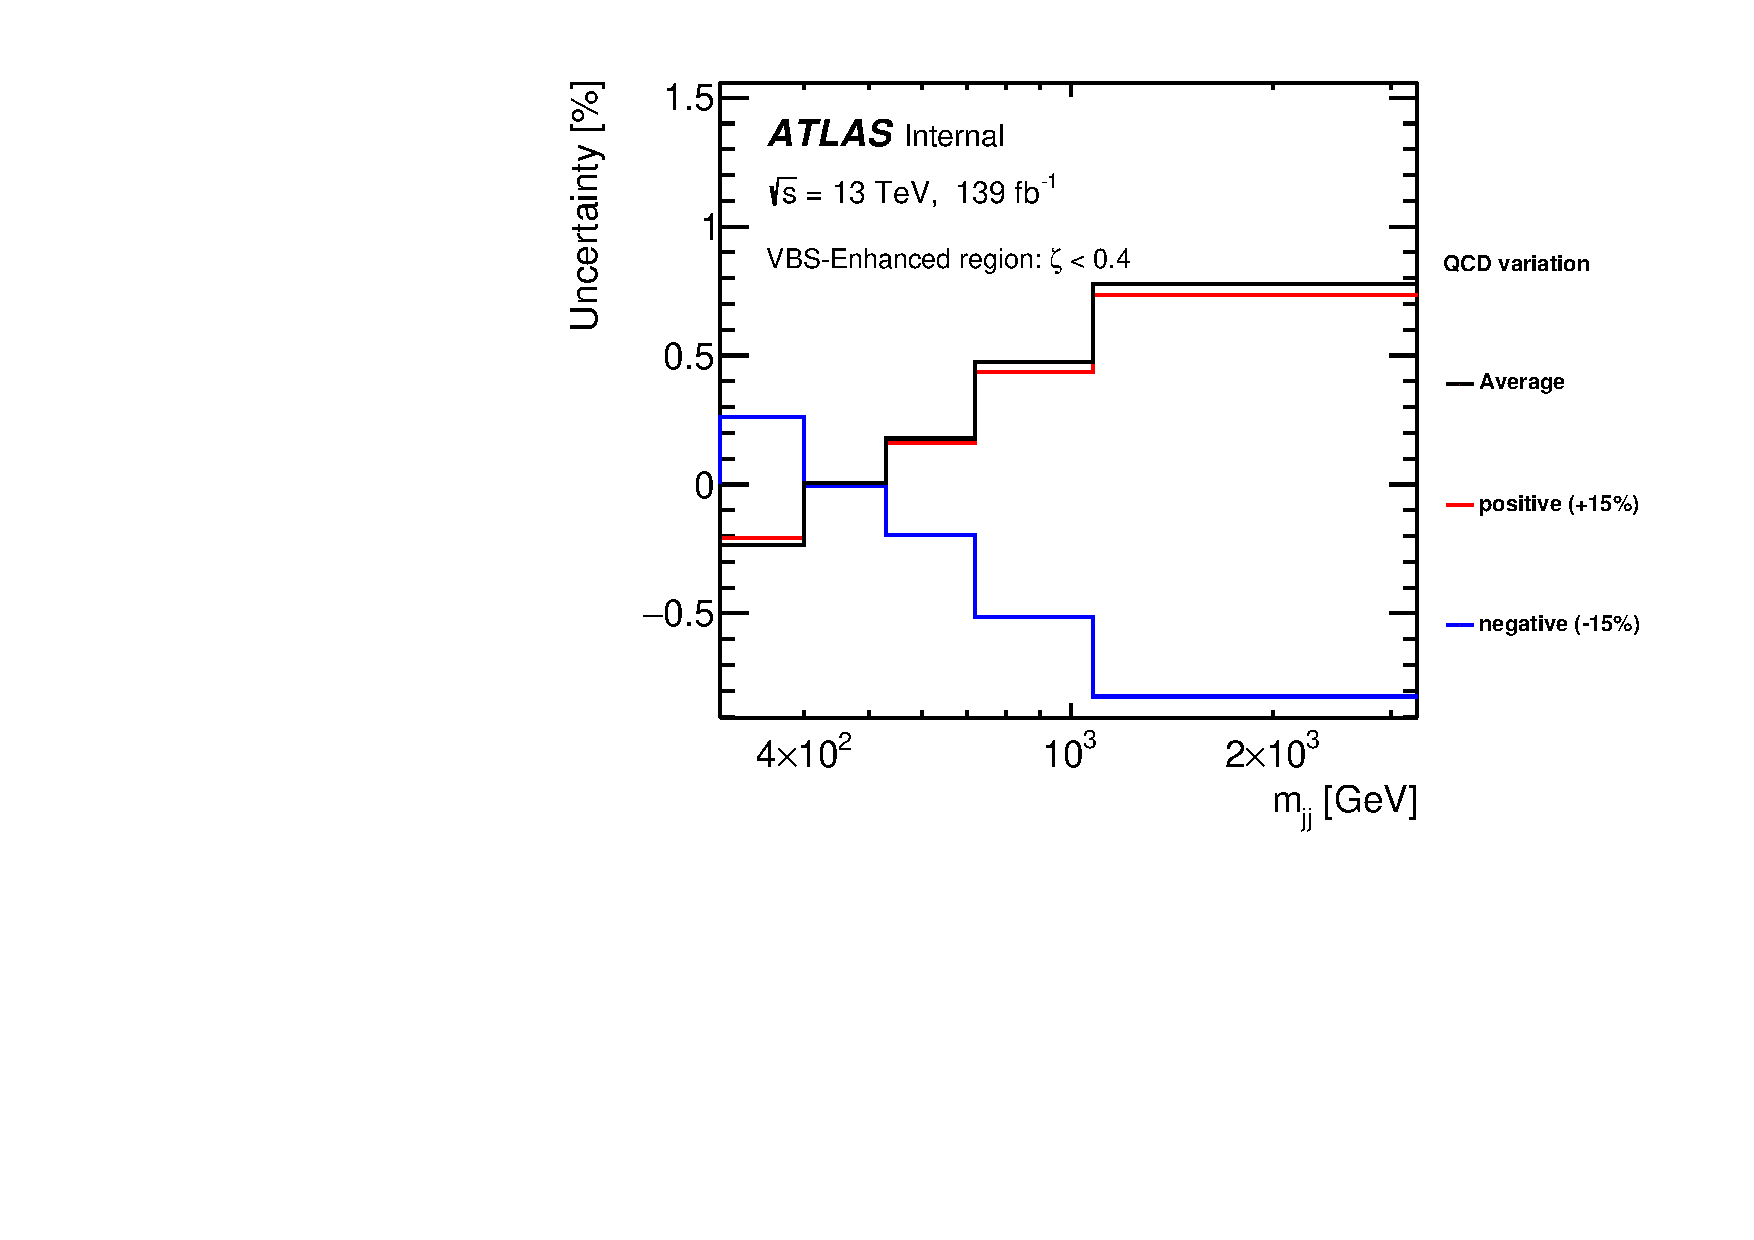
\includegraphics[width=.9\linewidth]{figures/Analysis/Unfolding/QCD_xsec_variation.pdf}
        \caption{ QCD cross-section is varied by $\pm  15\%$ \label{fig:unfolding_xsec_var_QCD} }
    \end{subfigure}
    \begin{subfigure}{.48\textwidth}
        \centering
        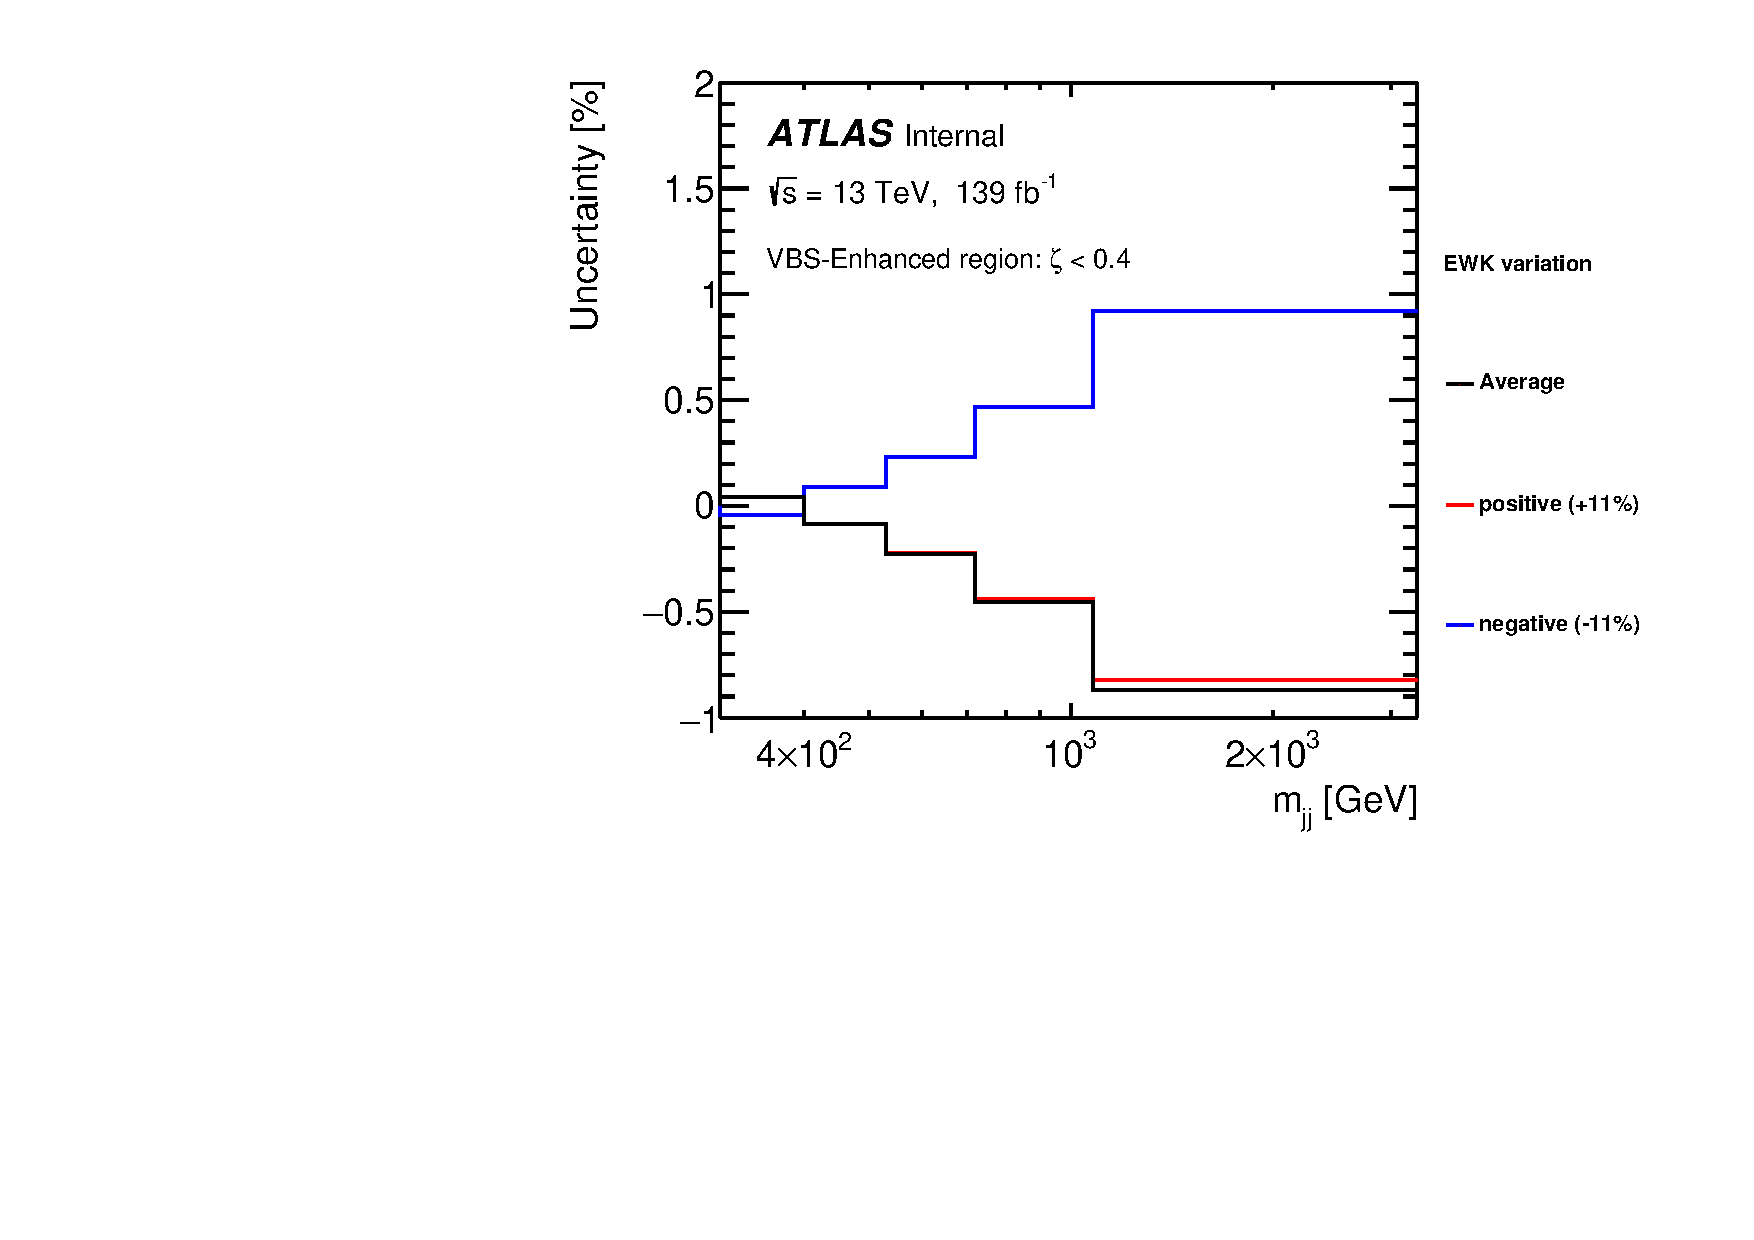
\includegraphics[width=.9\linewidth]{figures/Analysis/Unfolding/EWK_xsec_variation.pdf}
        \caption{ EWK cross-section is varied by $\pm 11\%$ \label{fig:unfolding_xsec_var_EWK}}
    \end{subfigure}
    \caption{ Unfolding validation using physics variation where parton-initiated QCD (left) or the EWK process cross-sections are varied. \label{fig:unfolding_xsec_var}}
\end{figure}

\subsection{Bias and Optimization}
\label{subsec:Bias}

The unfolded procedure relies on a prior value depending on the SM MC which naturally biases the unfolded cross-sections. With each iteration of unfolding, the algorithm improves the knowledge of the prior, thus, reducing the unfolding bias. However, with increasing number of iterations, the repeated bin migrations amplifies the statistical fluctuations in data, resulting in larger values of statistical uncertainties. Therefore, a finite number of iteration is chosen and the resulting unfolding bias is taken as the systematic uncertainty for the measurement. 

The unfolding bias is evaluated by the \textit{data-driven closure test}, where a pseudo dataset is developed utilizing the ratio of observed data and SM-predicted detector-level yield. First, for each observable the data and MC ratio is smoothed using Friedman's Super Smoother technique \cite{FriedmanSmoother}, fixing the end points to the value of ratio in the first and last bins. A reweighing function for each observable is developed to reweigh the SM fiducial- and detector-level yields. The reweighed detector-level signal-yield is then unfolded with the nominal unfolding inputs from SM and compared with the reweighed fiducial-level yield to get the final unfolding bias. Figure \ref{fig:unfolding_ddclosure} shows step-by-step procedure for the data-driven closure test. As shown by the ratio panel of figure \ref{fig:ddclosure_FinalBias}, unfolding bias of order $10\%$ is observed. 

\begin{figure}[htb]
    \centering
    \begin{subfigure}{.48\textwidth}
        \centering
        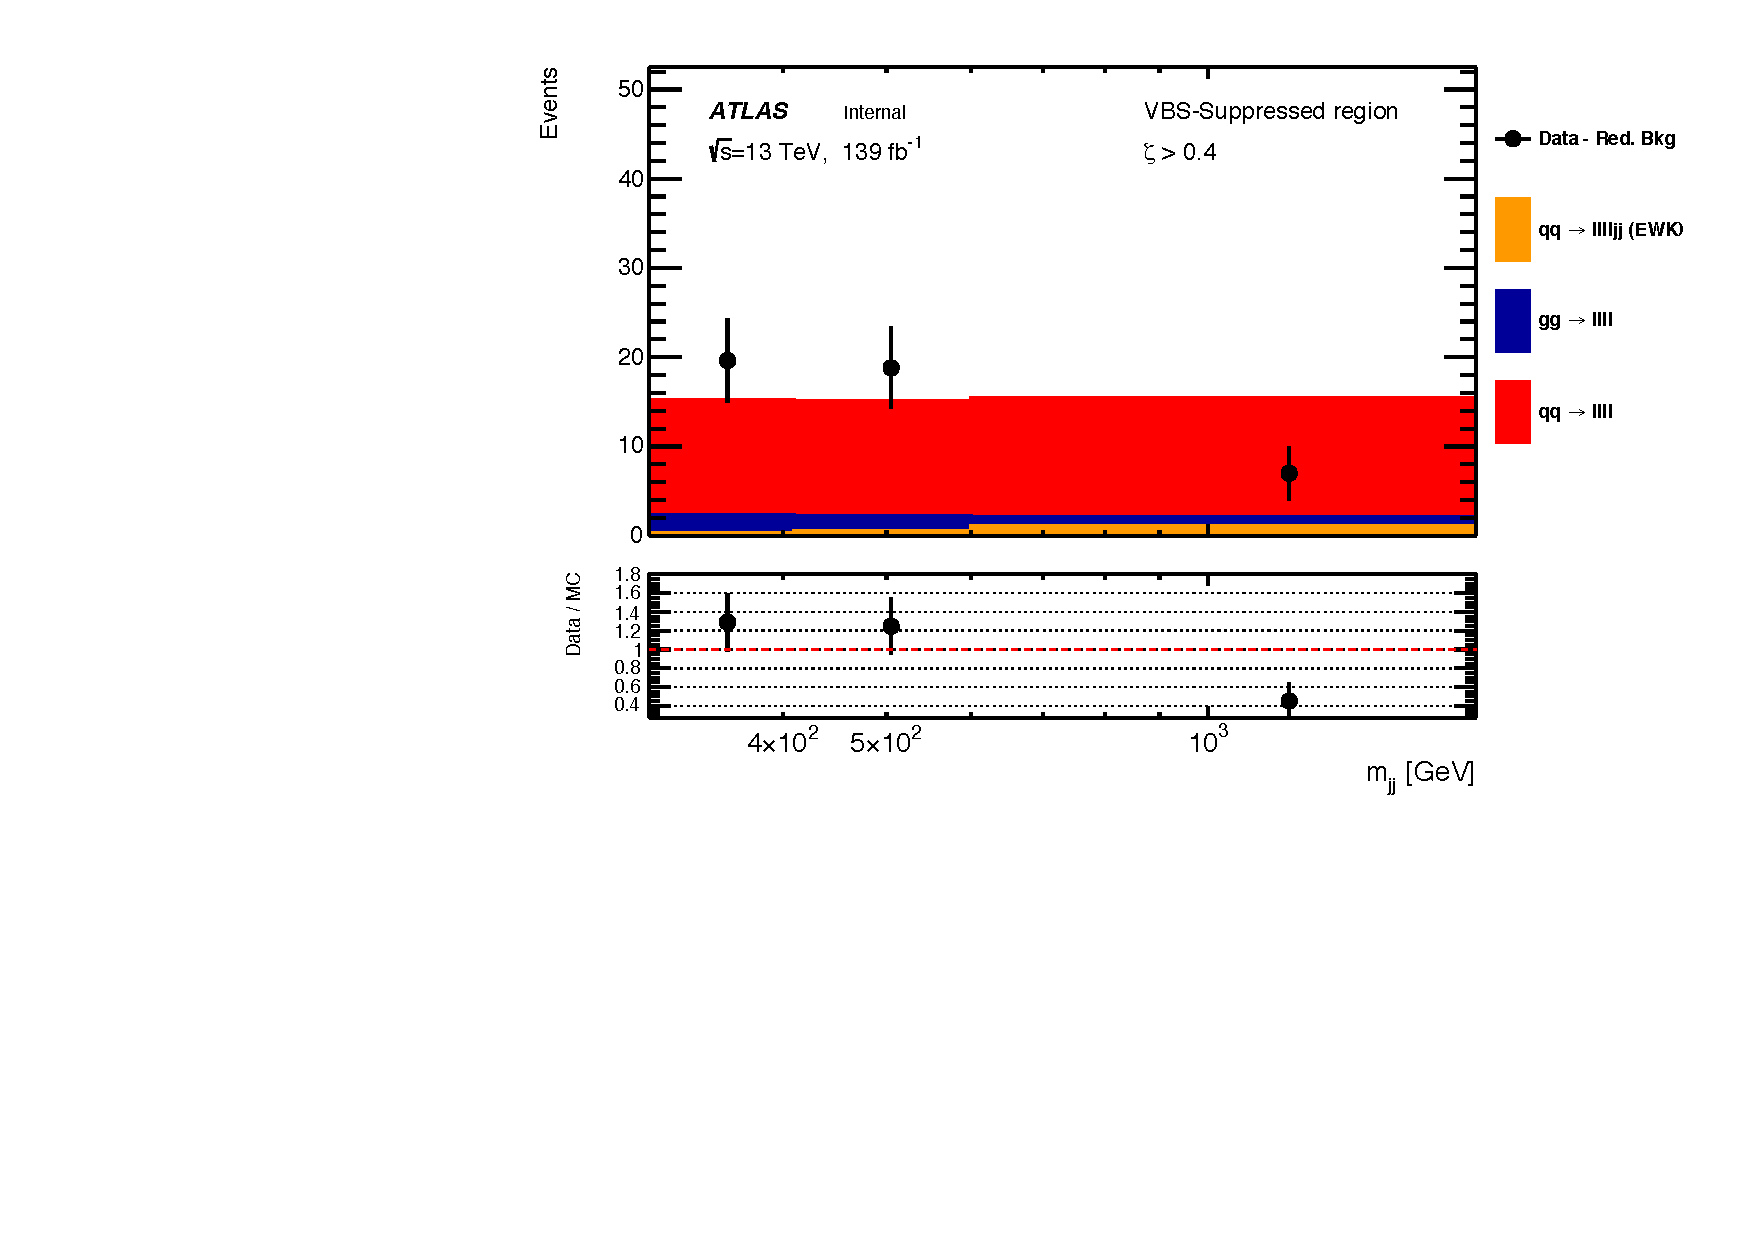
\includegraphics[width=.9\linewidth]{figures/Analysis/Unfolding/DDClosure_VBS_Suppressed_Ratio.pdf}
        \caption{ Data and MC for $m_{jj}$ \label{fig:ddclosure_DataMC}}
    \end{subfigure}
    \begin{subfigure}{.48\textwidth}
        \centering
        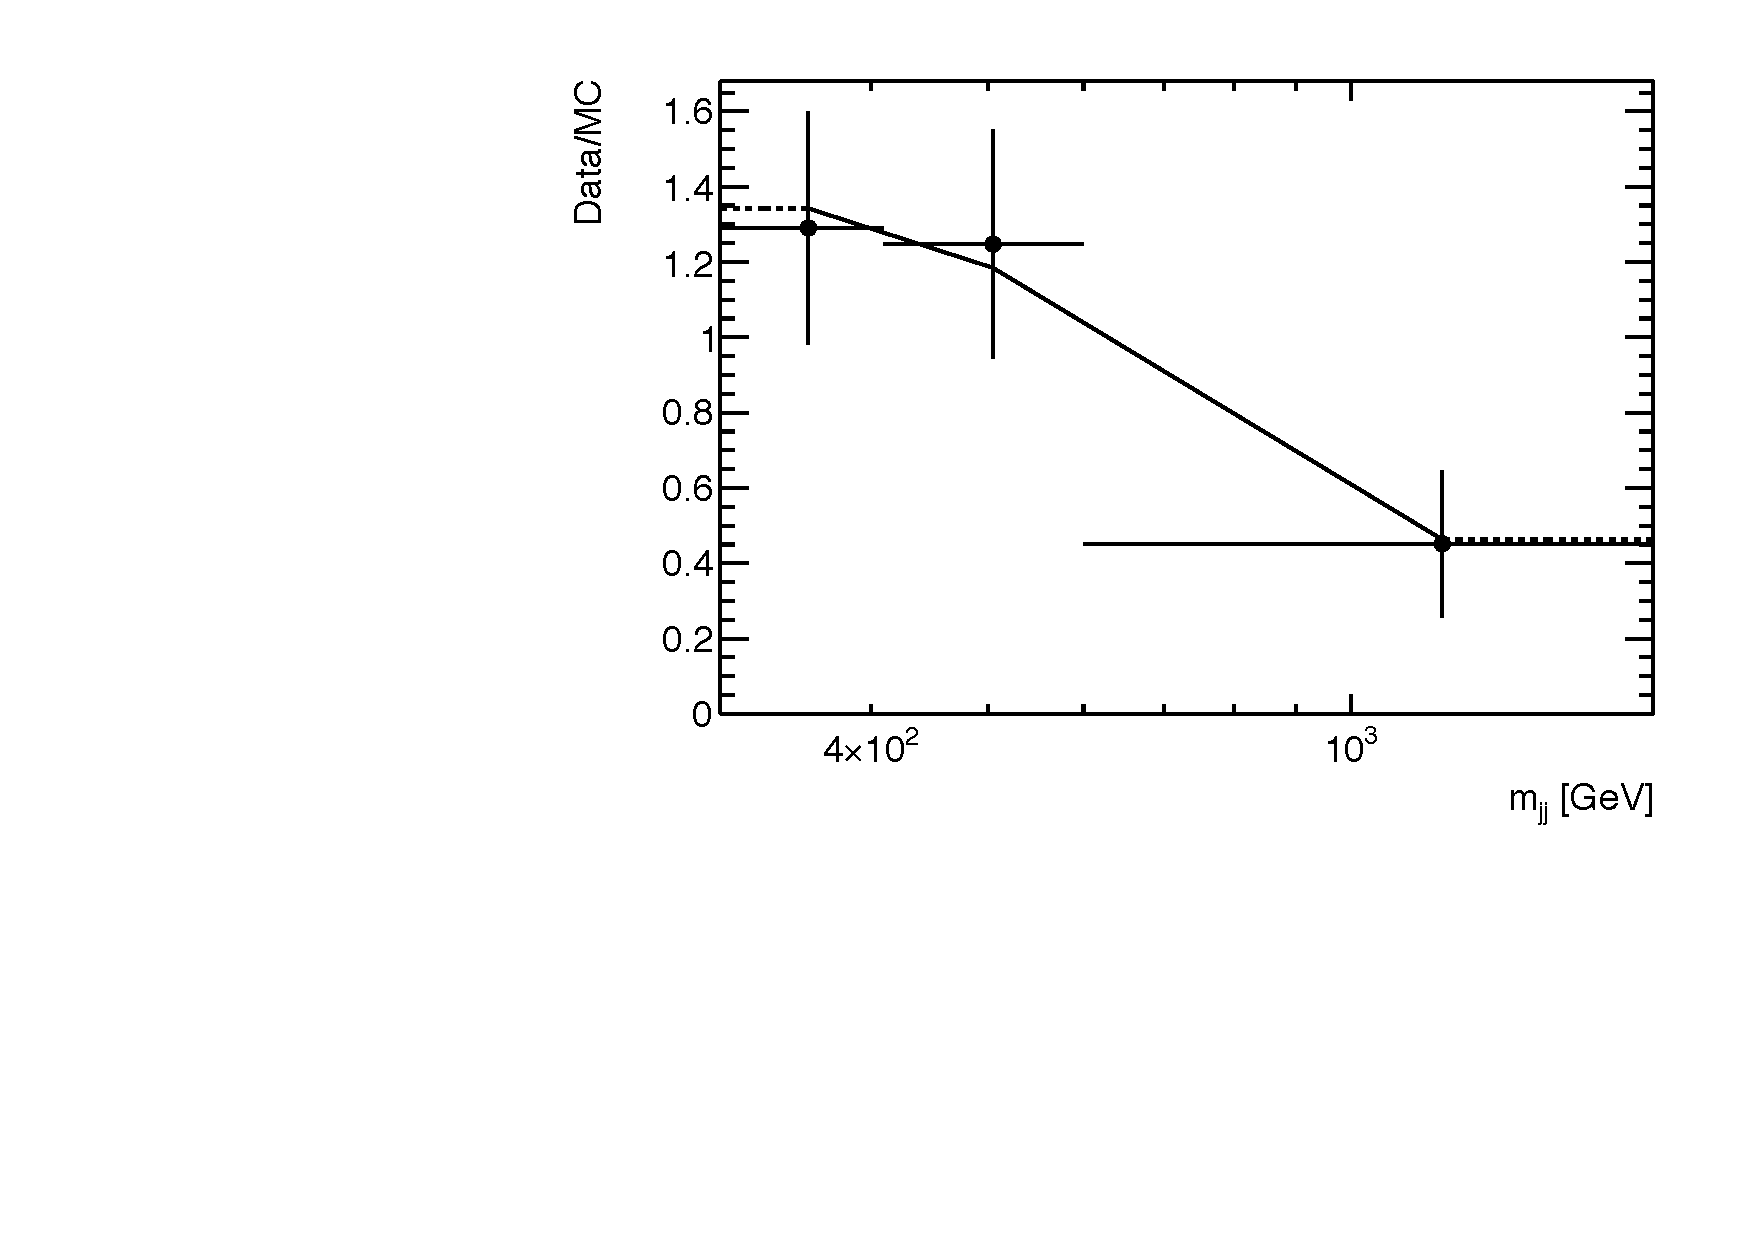
\includegraphics[width=.9\linewidth]{figures/Analysis/Unfolding/DDClosure_VBS_Suppressed_SmoothRatio.pdf}
        \caption{Smoothed ratio of Data and MC. \label{fig:ddclosure_DataMCSmooth} }
    \end{subfigure}\\
    \begin{subfigure}{.48\textwidth}
        \centering
        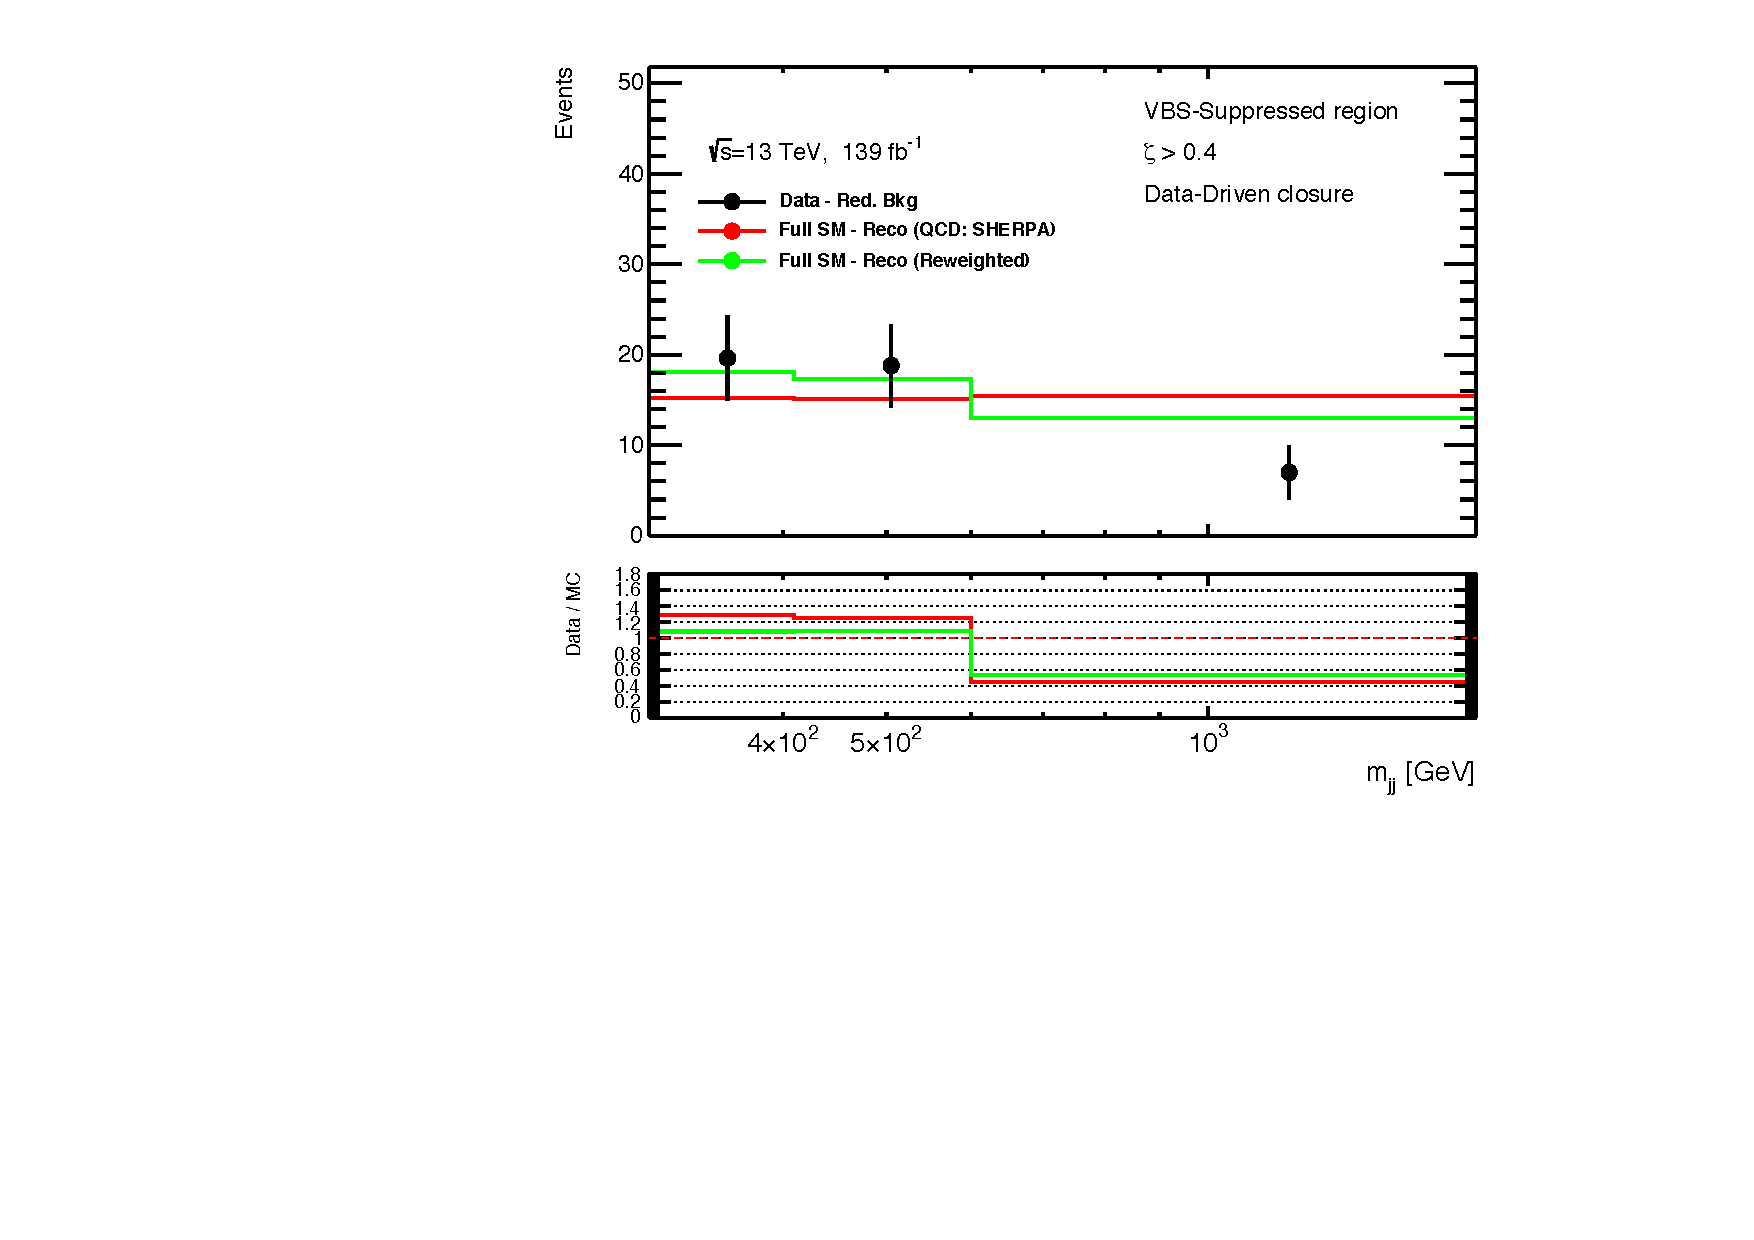
\includegraphics[width=.9\linewidth]{figures/Analysis/Unfolding/DDClosure_VBS_Suppressed_Reweighted.pdf}
        \caption{ Nominal SM (red) detector level yield and reweighted-detector level yield(green). \label{fig:ddclosure_DataMCReweighted} }
    \end{subfigure}
    \begin{subfigure}{.48\textwidth}
        \centering
        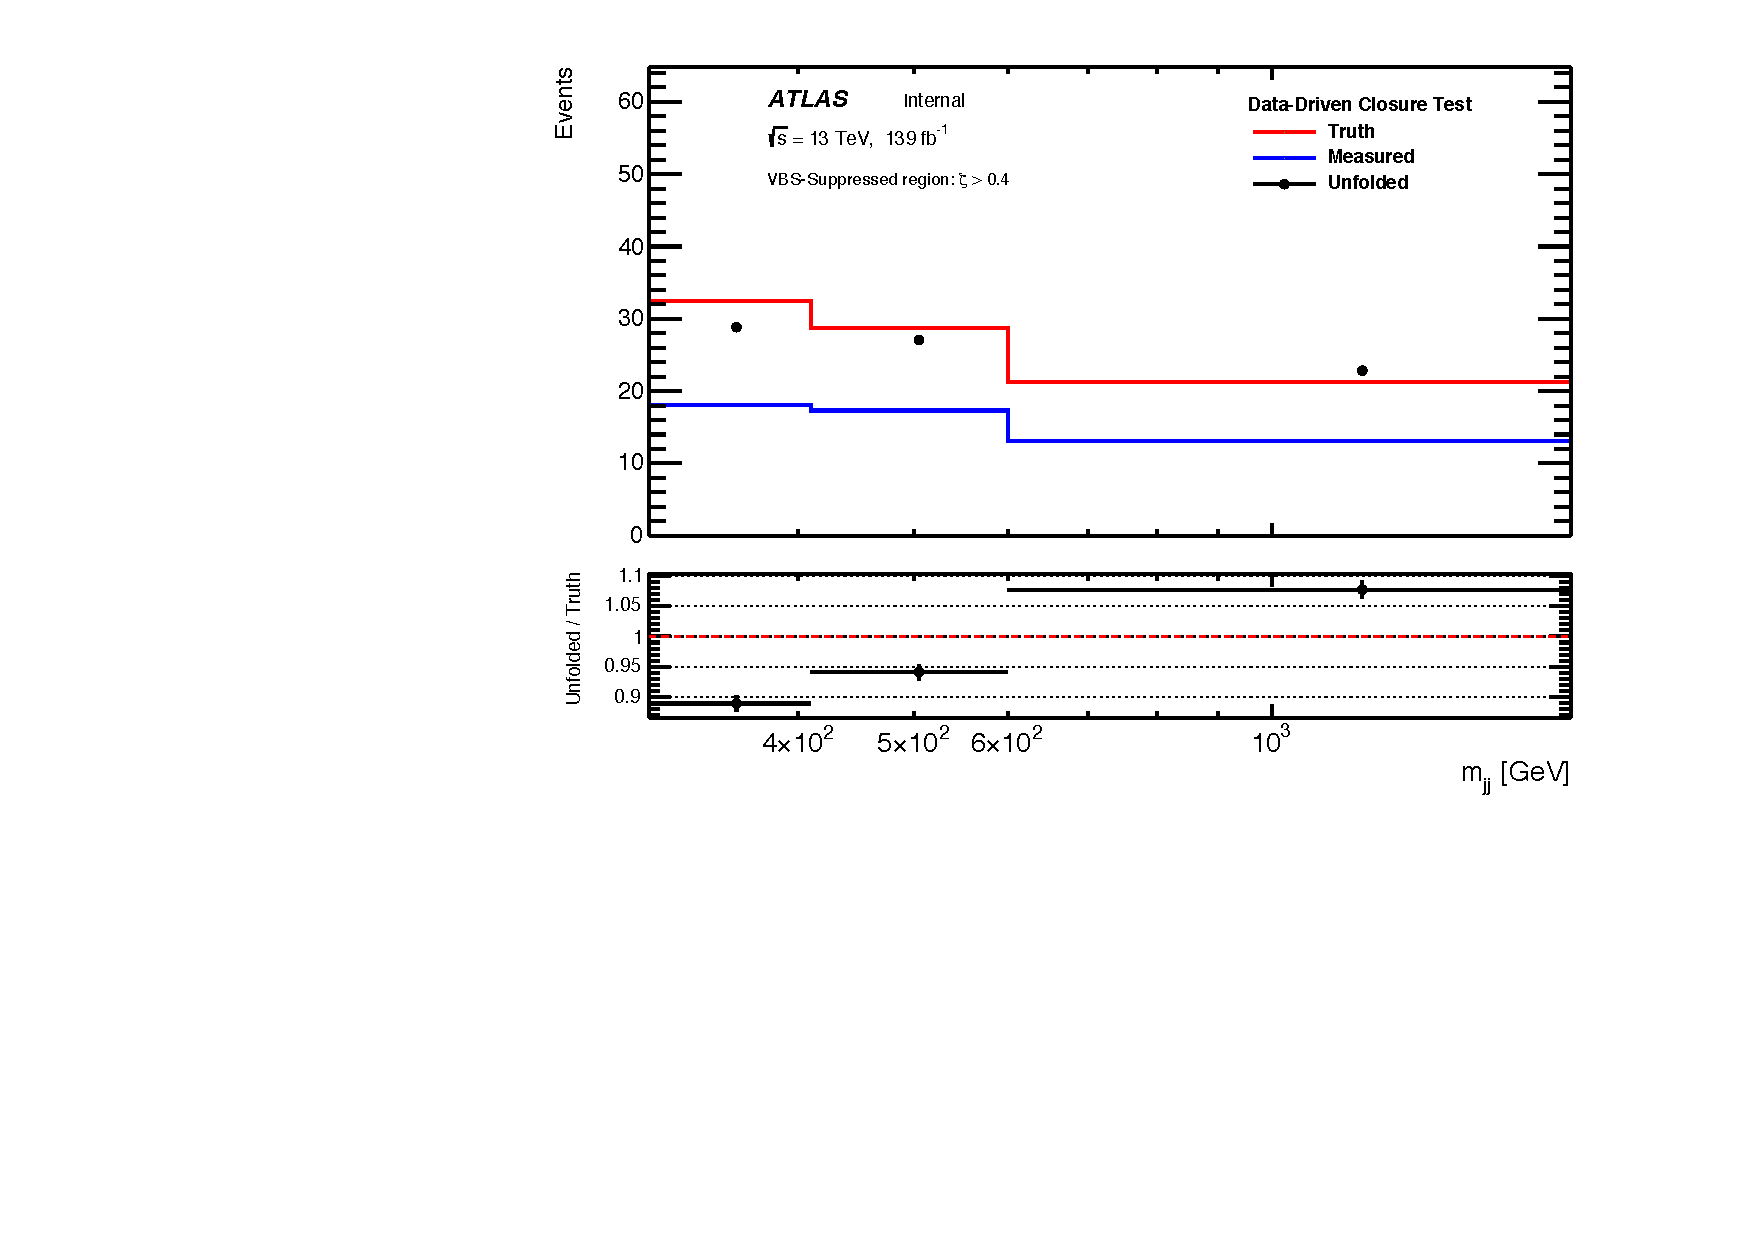
\includegraphics[width=.9\linewidth]{figures/Analysis/Unfolding/DDClosure_VBS_Suppressed_Bias.pdf}
        \caption{Unfolding bias. \label{fig:ddclosure_FinalBias} }
    \end{subfigure}
    \caption{ A step-by-step overview of the data driven closure test to get the unfolding bias.  \textcolor{red}{remake plots with ATLAS Label} \label{fig:unfolding_ddclosure}}
\end{figure}

The bias observed in figure \ref{fig:ddclosure_FinalBias} is obtained by using one number of iteration for unfolding. With a goal to reduce the unfolding bias, the data-driven closure test was repeated for several number of iterations. The resulting unfolding bias and systematic uncertainties up to $4$ iterations are shown in figure \ref{fig:BiasStatUnc}. As expected the unfolding bias decreases whereas the statistical uncertainty increases with the higher number of iteration. To balance between the statistical uncertainty and bias uncertainty, one number of iteration is chosen as optimal choice for the measurement.

\begin{figure}[htb]
    \centering
    \begin{subfigure}{.49\textwidth}
        \centering
        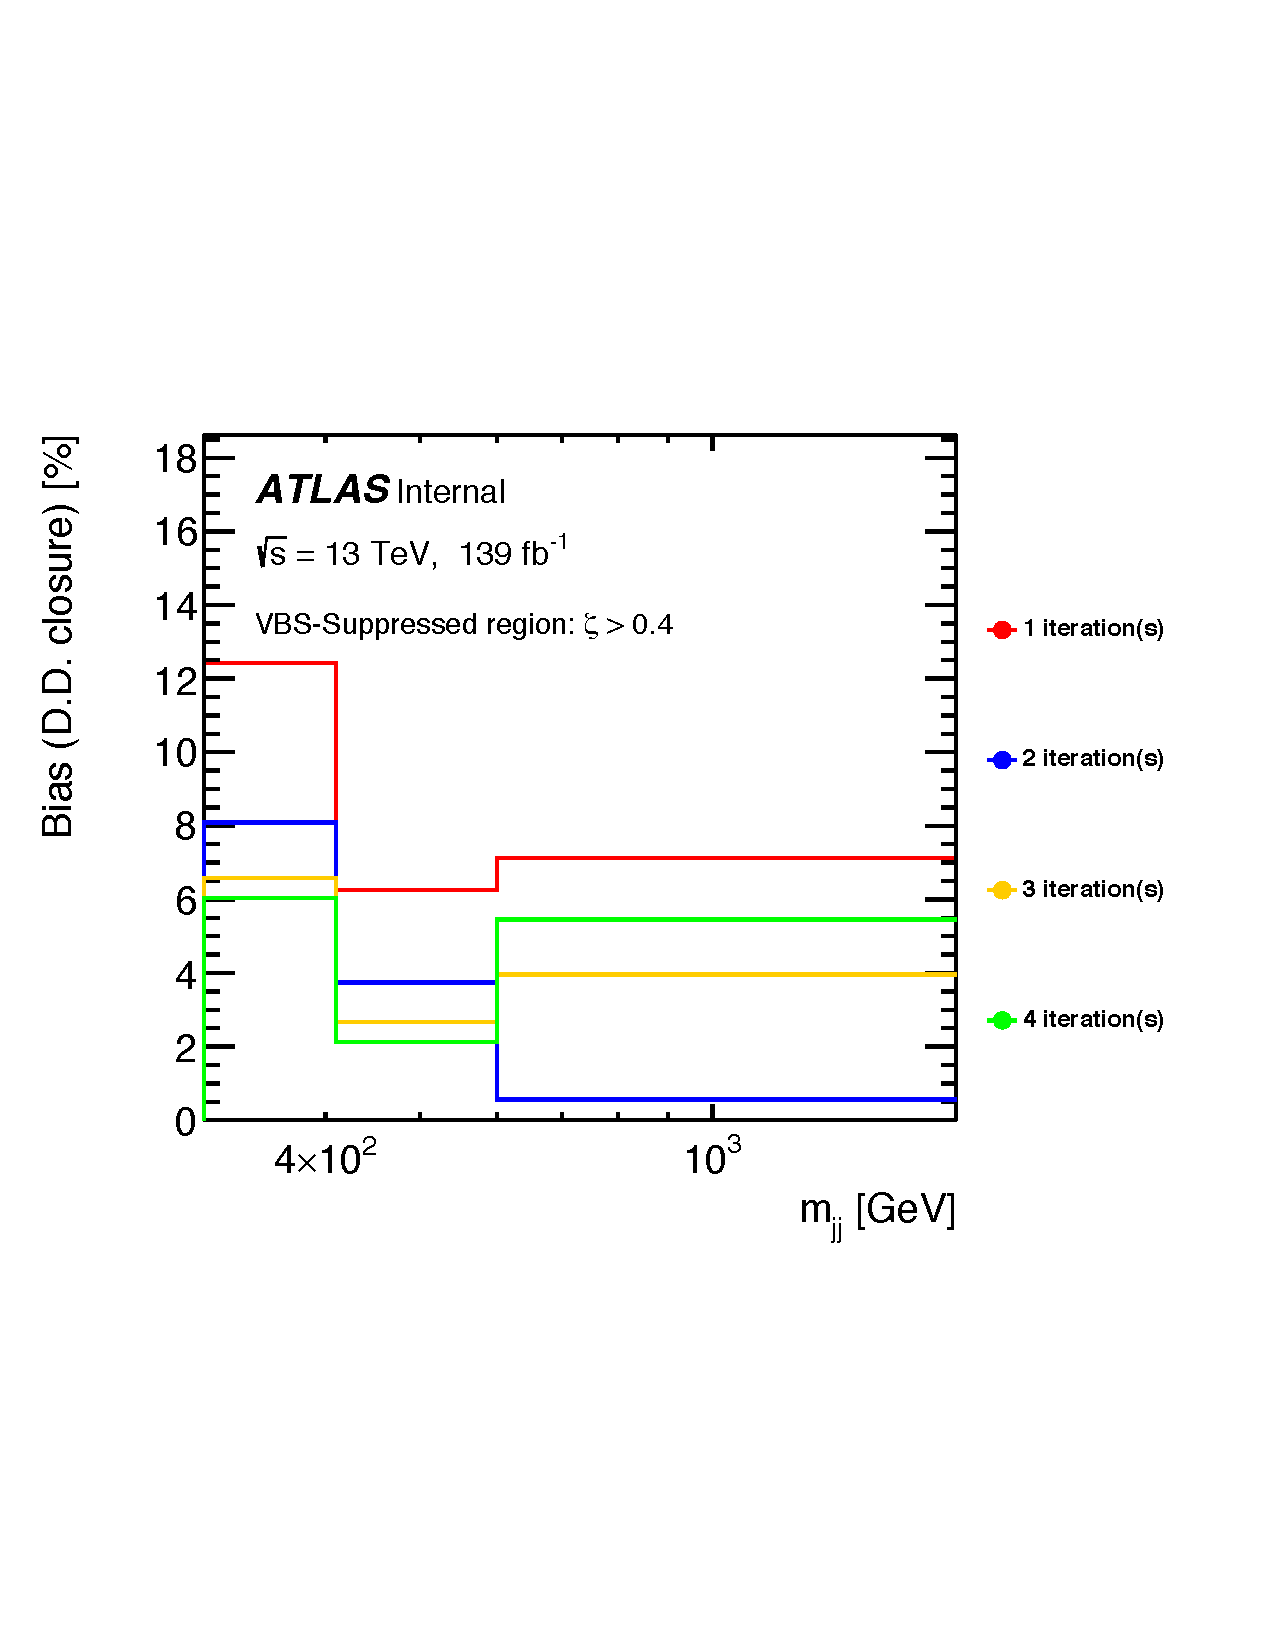
\includegraphics[width=.9\linewidth]{figures/Analysis/Unfolding/UnfoldingBiasIteration.pdf}
       % \caption{ Unfolding bias \label{fig:UnfoldingBiasIteration} }
    \end{subfigure}
    \begin{subfigure}{.49\textwidth}
        \centering
        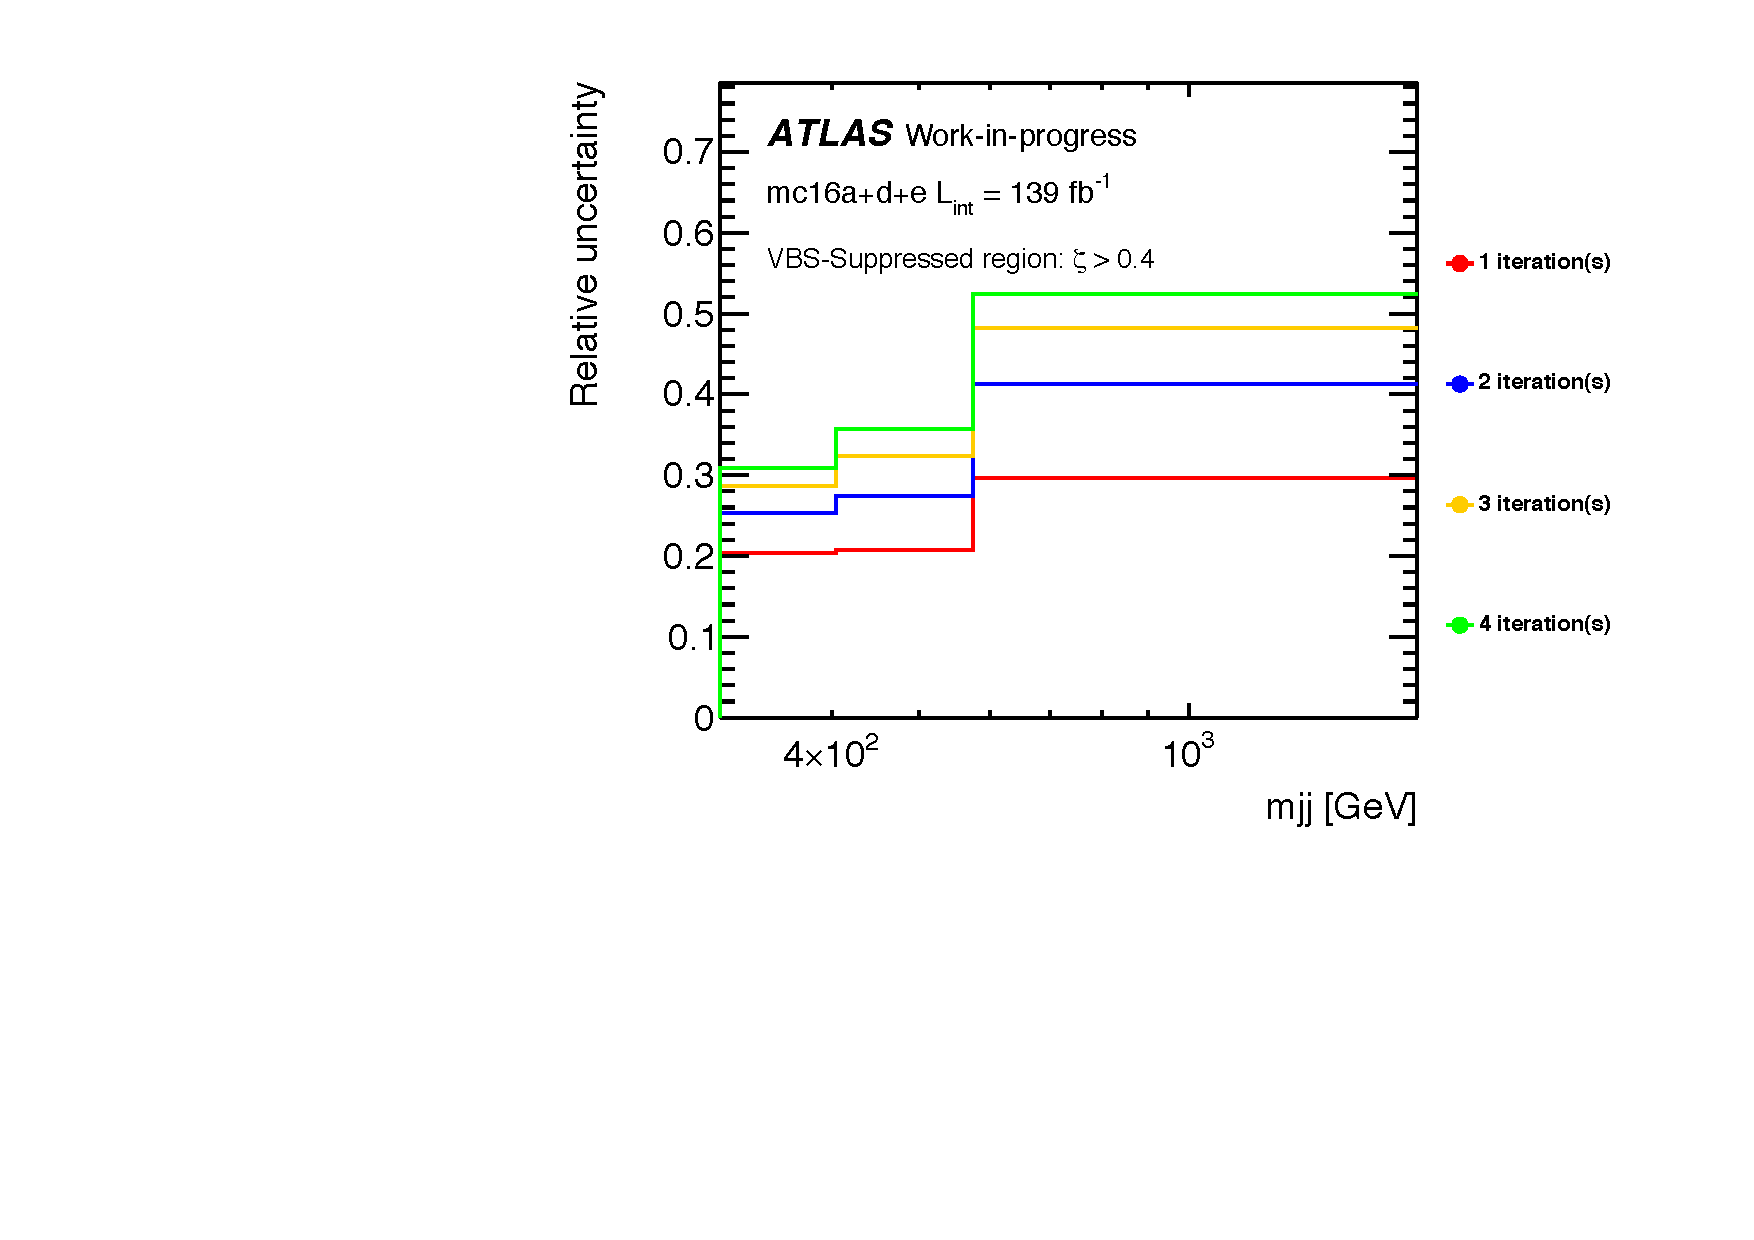
\includegraphics[width=.9\linewidth]{figures/Analysis/Unfolding/StatUnc_Sup.pdf}
        %\caption{ Statistical uncertainty \label{fig:UnfoldingStatUnc}}
    \end{subfigure}
    \caption{ Unfolding bias (left) and statistical uncertainty (right) with up to $4$ unfolding iterations as a function of $m_{jj}$ in VBS-Suppressed region. \label{fig:BiasStatUnc}}
\end{figure}

Unfolding bias is the largest source of the systematic uncertainty of the analysis and is studied in detail using a MC-driven toy studies to understand the source. The observed large bias is from detector-level pileup jets at lower $p_{T}$ or higher $\eta$ that are not part of the fiducial phase space. The jet-vertex-tagger and forward-jet-vertex-tagger has lower efficiency to select the hard scattering jets at lower $p_{T}$ or higher $\eta$, thus resulting in more \textit{fiducial-fake-event} contamination. The additional MC-based studies on the unfolding bias are summarized in Appendix \ref{Appendix:Unfolding_bias}. 
